%\section{Introduction}
\begin{figure}[h]
\vspace*{-0mm}
\hspace*{-6mm}
	\centering
	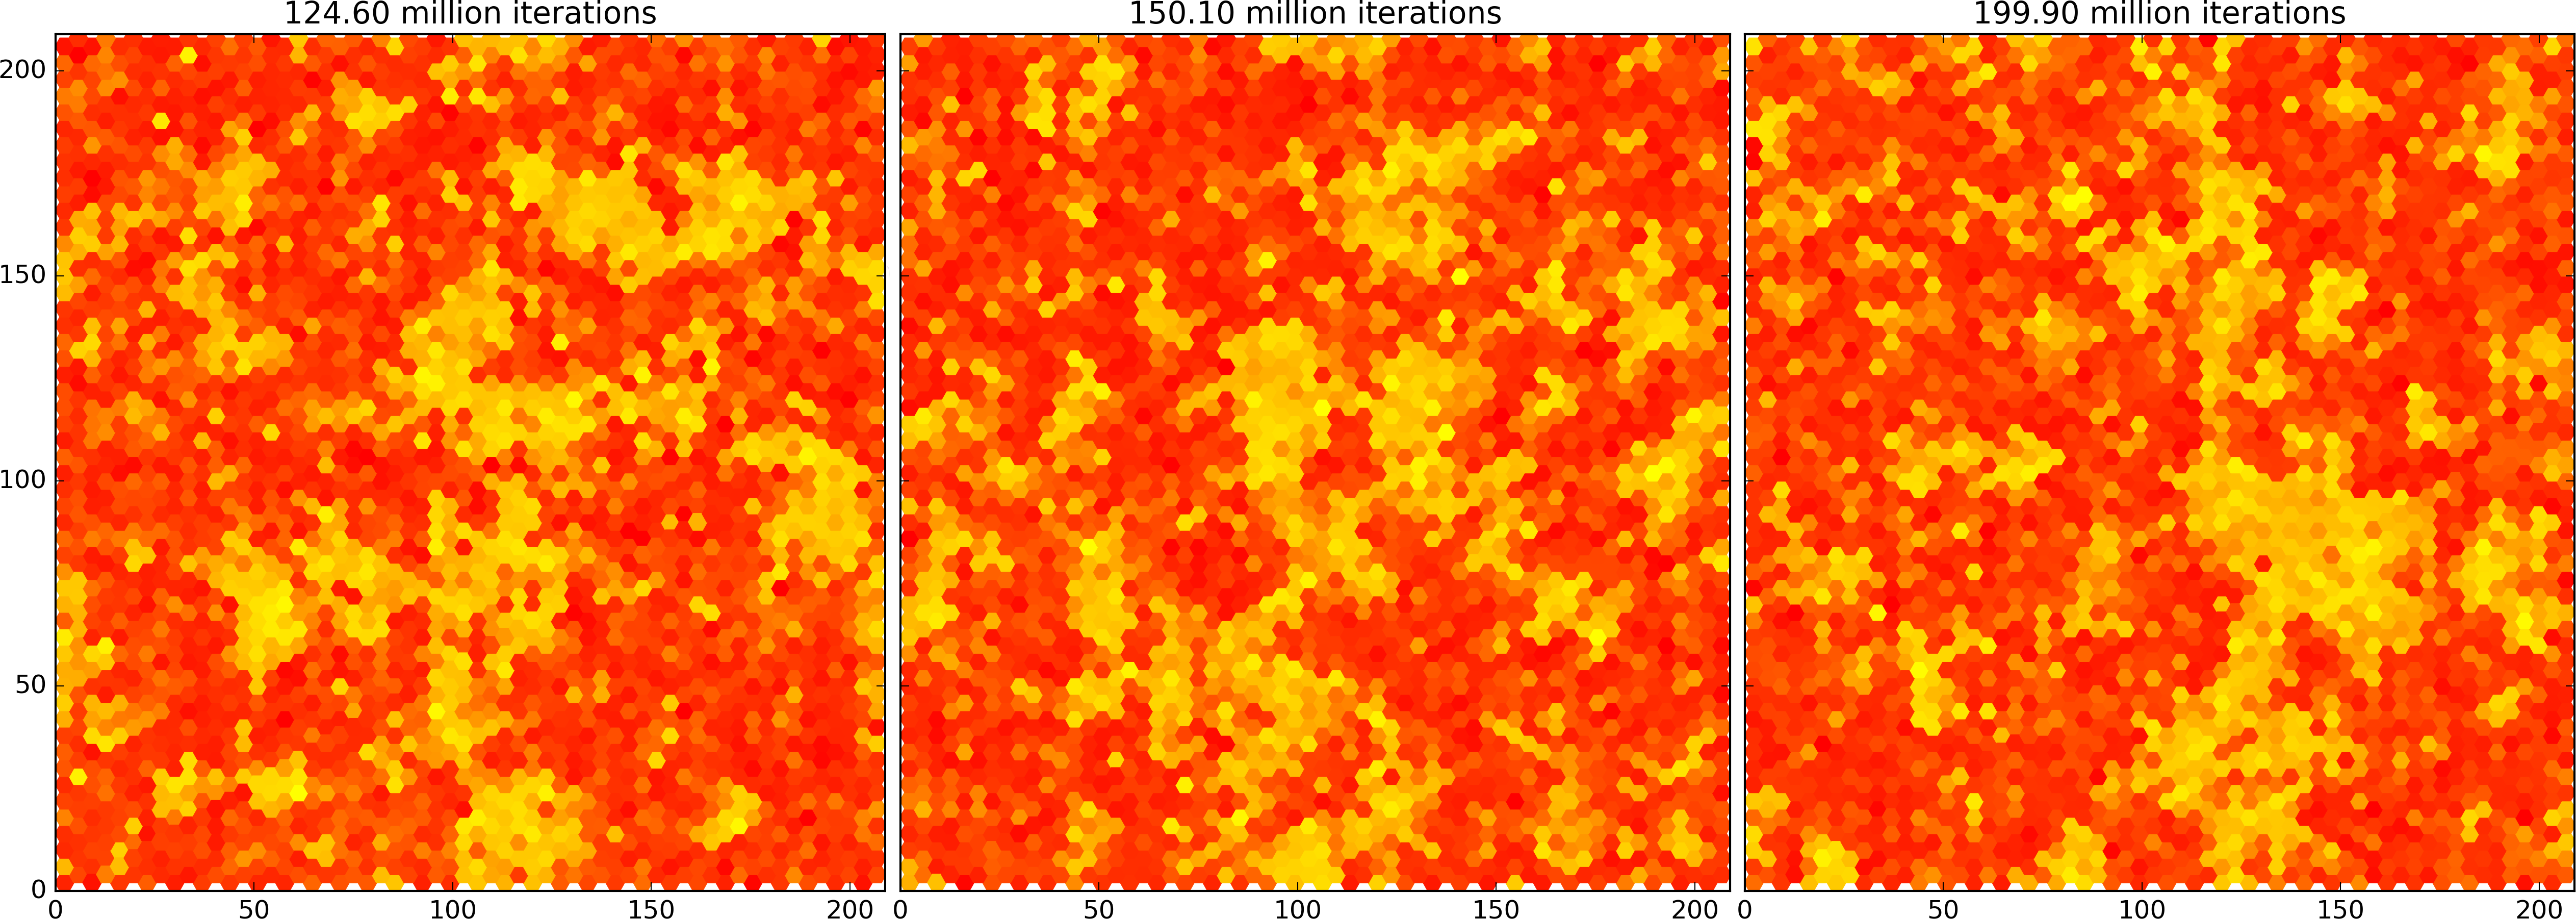
\includegraphics[width=\textwidth]{renorm}
	\caption{
	%\tiny	
	\scriptsize
	Here a simulation of a 2d fluid near the critical point is presented. The three images are the same fluid seperated in time. The interface between liquid and gas evolves in time as each globule will interact with neighboring globules. If the temperature is increased past the critical point, the globules shrink in size to the point the plots appear as white noise.}
	\label{fig:renorm}
\end{figure}

The liquid-vapor phase coexistence can be found by just placing some liquid into a sealed container. Some of the liquid will evaporate into the jar creating a vapor pressure. Provided we placed enough liquid into the jar, the system will now contain both a liquid and a vapor at the same time. By sealing the liquid into a jar, we have forced the pressure of the liquid to be the as the pressure of the gas. By allowing the atoms to swap between the liquid and gas phase, we have also allowed the chemical potential of the liquid to be the same as that of the gas.

Although we can find the phase coexistence by physically sealing a liquid in a jar, an equivalent computational method is to use an empirically determined fluid model which we can use to run simulations that also equalize the pressur
e and chemical potential. The problem with the computational method is the empirical model requires fitting a few parameters to data, data which probably already includes points on the phase coexistence curve. The main benefit to the computational approach is that once the empirical parameters are found, we can then create the phase coexistence of a mixture of fluids using the previously determined parameters.

One of the difficulties with the computer simulations is computation time. A simulation with a handful of atoms can be finished within 20 minutes, yet a simulation with a 100 atoms can take as long as 4 days. To recreate the phase coexistence graph requires setting the pressure and chemical potential of both phases equal to each other, but this is equivalent to plotting the free energy as a function of density and searching for a common cotangent. For even a simulation that uses a small box, the problem is plotting free energy as a function of density requires many simulations at various densities; some simulations containing only a handful of atoms while other simulations containing as much as a couple hundred atoms. Total computation time for 10 computer cores to create the free energy as a function of density graph can take as long as three weeks.

Naturally there is a tradeoff between a realistic computation time for a project and how realistic the results are going to be. The simulations use periodic boundary conditions which is just the thermodynamic way of saying the boundary should not affect the bulk properties. The key part being whatever is in the simulation is considered the bulk, which is a problem since a small simulation can hardly be considered the bulk. To get around this problem, the simulation size is usually increased until the simulation does represent the bulk. 

Normally increasing the simulation size is just fine, but there is a regime where the bulk properties depend on length scales of the order of a millimeter. This regime occurs near the critical point where the liquid density approaches that of the vapor. Normally the liquid and vapor are entirely seperated due to the surface tension. However; as the system approaches the critical point, the surface tension approaches zero which means the liquid and vapor will start to mix. Although figure 1 shows an extreme example of a liquid completely mixing with vapor, even under normal circumstances there exist natural fluctuations in the density of either phase. It just so happens that these fluctuations are significant as the density of the liquid approaches the density of the gas at the critical point. Basically the fluctuations within each phase would normally be rather small, but near the critical point the fluctuations are relatively big since the gas and liquid phases are morphing into each other. This is a problem since it requires the simulations to be about the same size as that of the largest fluctuation. For example, a 1mm length box would contain roughly $10^{19}$ atoms, which would require an unfeasible computation time.

Renormalization group theory(RGT) can be applied to get around this large fluctuation problem. Simply put, RGT is a method in which fine details are omitted from calculations while still maintaining accuracy. This is done by transforming the original partition funciton into a smaller partition function, but the smaller system is renormalized to the original parition function. [add details...]

In particular, RGT is applied through an interaction wave length. The zeroth order is just the ideal gas term in which all atoms only interact with the walls of the enclosure. The next order is applied via SAFT-VR in which a mean interaction and an approximate wavelength interaction is applied. Longer wavelength interactions can then be applied using RGT via a iterative method that steadily increases the size of the box.

The main problem this project addresses is the transition from SAFT-VR to the application of RGT. Within RGT there is an arbitrary base wavelength L which is usually fit to the data. However; this arbitrary wavelength shouldn't really be an arbitrary parameter as SAFT-VR already includes interactions at some unknown wavelength. This project attempts to find the base wavelength that SAFT-VR implements, and tests how the results of RGT change when using this base wavelength.

The base wavelength is found by using Monte Carlo Markov Chain (MCMC) simulations at various box sizes. The idea is that a MCMC simulation using a fixed box size of $L_0$ will incorporate interactions at this box size. The box size is then varied until the results from the MCMC simulations fit the results from SAFT-VR. Once the optimal box size is found, RGT is implemented using this optimal box size and the results are compared to previous results.

